\documentclass[tikz,border=3pt]{standalone}
\usepackage[T1]{fontenc}
\usepackage{mathpazo}
\usepackage{amsmath}
\usetikzlibrary{arrows.meta,positioning,calc,decorations.pathreplacing}

\definecolor{pfblue}{HTML}{DCEAF7}
\definecolor{pfteal}{HTML}{DDEFE8}
\definecolor{pfgold}{HTML}{F6E9C6}
\definecolor{pfviolet}{HTML}{E9E1F0}
\definecolor{pfslate}{HTML}{E4EBF1}
\definecolor{pforange}{HTML}{F2D8C6}
\definecolor{pfink}{HTML}{202A34}
\definecolor{pfmuted}{HTML}{596674}

\begin{document}
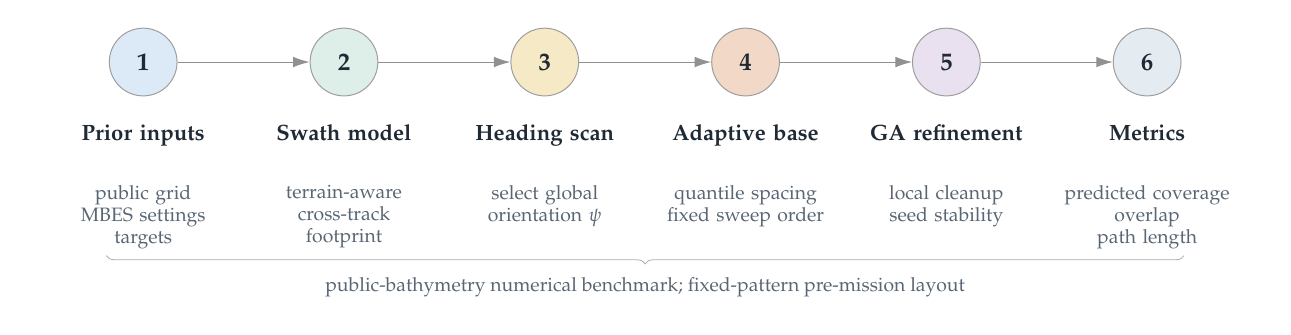
\begin{tikzpicture}[
    font=\rmfamily,
    >=Latex,
    pstep/.style={
        circle,
        draw=black!38,
        line width=0.36pt,
        minimum size=8.6mm,
        inner sep=0pt,
        font=\bfseries\small,
        text=pfink
    },
    label/.style={
        align=center,
        text width=27mm,
        font=\bfseries\footnotesize,
        text=pfink
    },
    sublabel/.style={
        align=center,
        text width=27mm,
        font=\scriptsize,
        text=pfmuted
    },
    arrow/.style={
        -{Latex[length=2.1mm,width=1.35mm]},
        draw=black!43,
        line width=0.38pt
    },
    note/.style={
        align=center,
        font=\scriptsize,
        text=pfmuted
    }
]

\node[pstep, fill=pfblue] (s1) at (0,0) {1};
\node[pstep, fill=pfteal] (s2) at (2.55,0) {2};
\node[pstep, fill=pfgold] (s3) at (5.10,0) {3};
\node[pstep, fill=pforange] (s4) at (7.65,0) {4};
\node[pstep, fill=pfviolet] (s5) at (10.20,0) {5};
\node[pstep, fill=pfslate] (s6) at (12.75,0) {6};

\foreach \a/\b in {s1/s2,s2/s3,s3/s4,s4/s5,s5/s6}
    \draw[arrow] (\a.east) -- (\b.west);

\node[label, below=2.4mm of s1] {Prior inputs};
\node[sublabel, below=10.0mm of s1] {public grid\\MBES settings\\targets};

\node[label, below=2.4mm of s2] {Swath model};
\node[sublabel, below=10.0mm of s2] {terrain-aware\\cross-track\\footprint};

\node[label, below=2.4mm of s3] {Heading scan};
\node[sublabel, below=10.0mm of s3] {select global\\orientation \(\psi\)};

\node[label, below=2.4mm of s4] {Adaptive base};
\node[sublabel, below=10.0mm of s4] {quantile spacing\\fixed sweep order};

\node[label, below=2.4mm of s5] {GA refinement};
\node[sublabel, below=10.0mm of s5] {local cleanup\\seed stability};

\node[label, below=2.4mm of s6] {Metrics};
\node[sublabel, below=10.0mm of s6] {predicted coverage\\overlap\\path length};

\draw[decorate,decoration={brace,amplitude=3.0pt,mirror},draw=black!32,line width=0.30pt]
    ($(s1.south west)+(-0.16,-2.15)$) -- ($(s6.south east)+(0.16,-2.15)$)
    node[midway,below=4.5pt,note] {public-bathymetry numerical benchmark; fixed-pattern pre-mission layout};

\end{tikzpicture}
\end{document}
